\section{Approach Overview}
\label{sec:overview}

\begin{figure*}[ht]
 \centering
 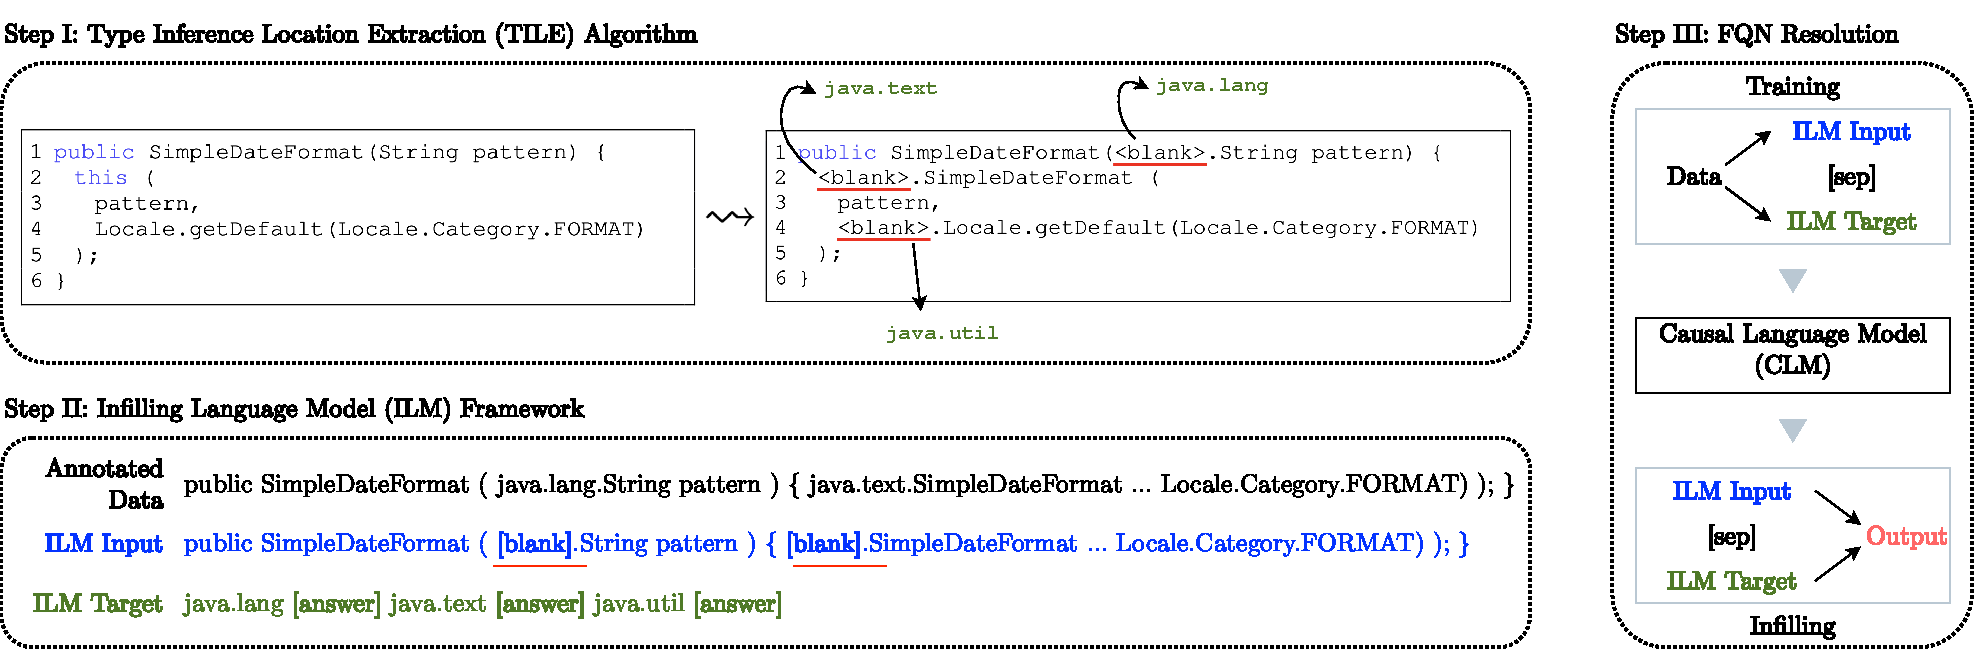
\includegraphics[width=0.95\textwidth]{overview-ilm.pdf}
 \caption{Illustrated: A general overview of \tool approach for resolving fully-qualified names.}
 \label{fig:approach}
\end{figure*}

Fig.~\ref{fig:approach} illustrates the general overview of {\tool}. It has two primary components, the first of which is the {\em Type Inference Location Extraction} (TILE) algorithm. Given a code snippet, TILE analyzes it to identify all locations where an API name needs to be expanded. Next, at each of these type inference locations, it inserts a \code{<blank>} token to represent the missing part of the fully-qualified name (FQN). Let us refer to the resulting \code{<blank>} inserted code snippet as \code{<blank>}-code.

The goal of the next stage is to infer all FQNs corresponding to the \code{<blank>} tokens in the \code{<blank>}-code. As discussed in Section~\ref{sec:key}, an effective FQN resolution solution incorporates the inter-connections between API and program elements. Thus, we consider the Infilling Language Model (ILM) introduced by Donahue et al.~\cite{} as the next component in our approach. Unlike standard language models (LMs), the ILM framework is capable of incorporating context on both sides of the blank, which in turn facilitates inter-API dependency learning. Such contextual knowledge coupled with ILM's ability to effectively predict missing spans of text helps \tool derive FQNs at all relevant API locations.


%%%\begin{figure}[t] %[!htp]
%%%	\centering
%%%	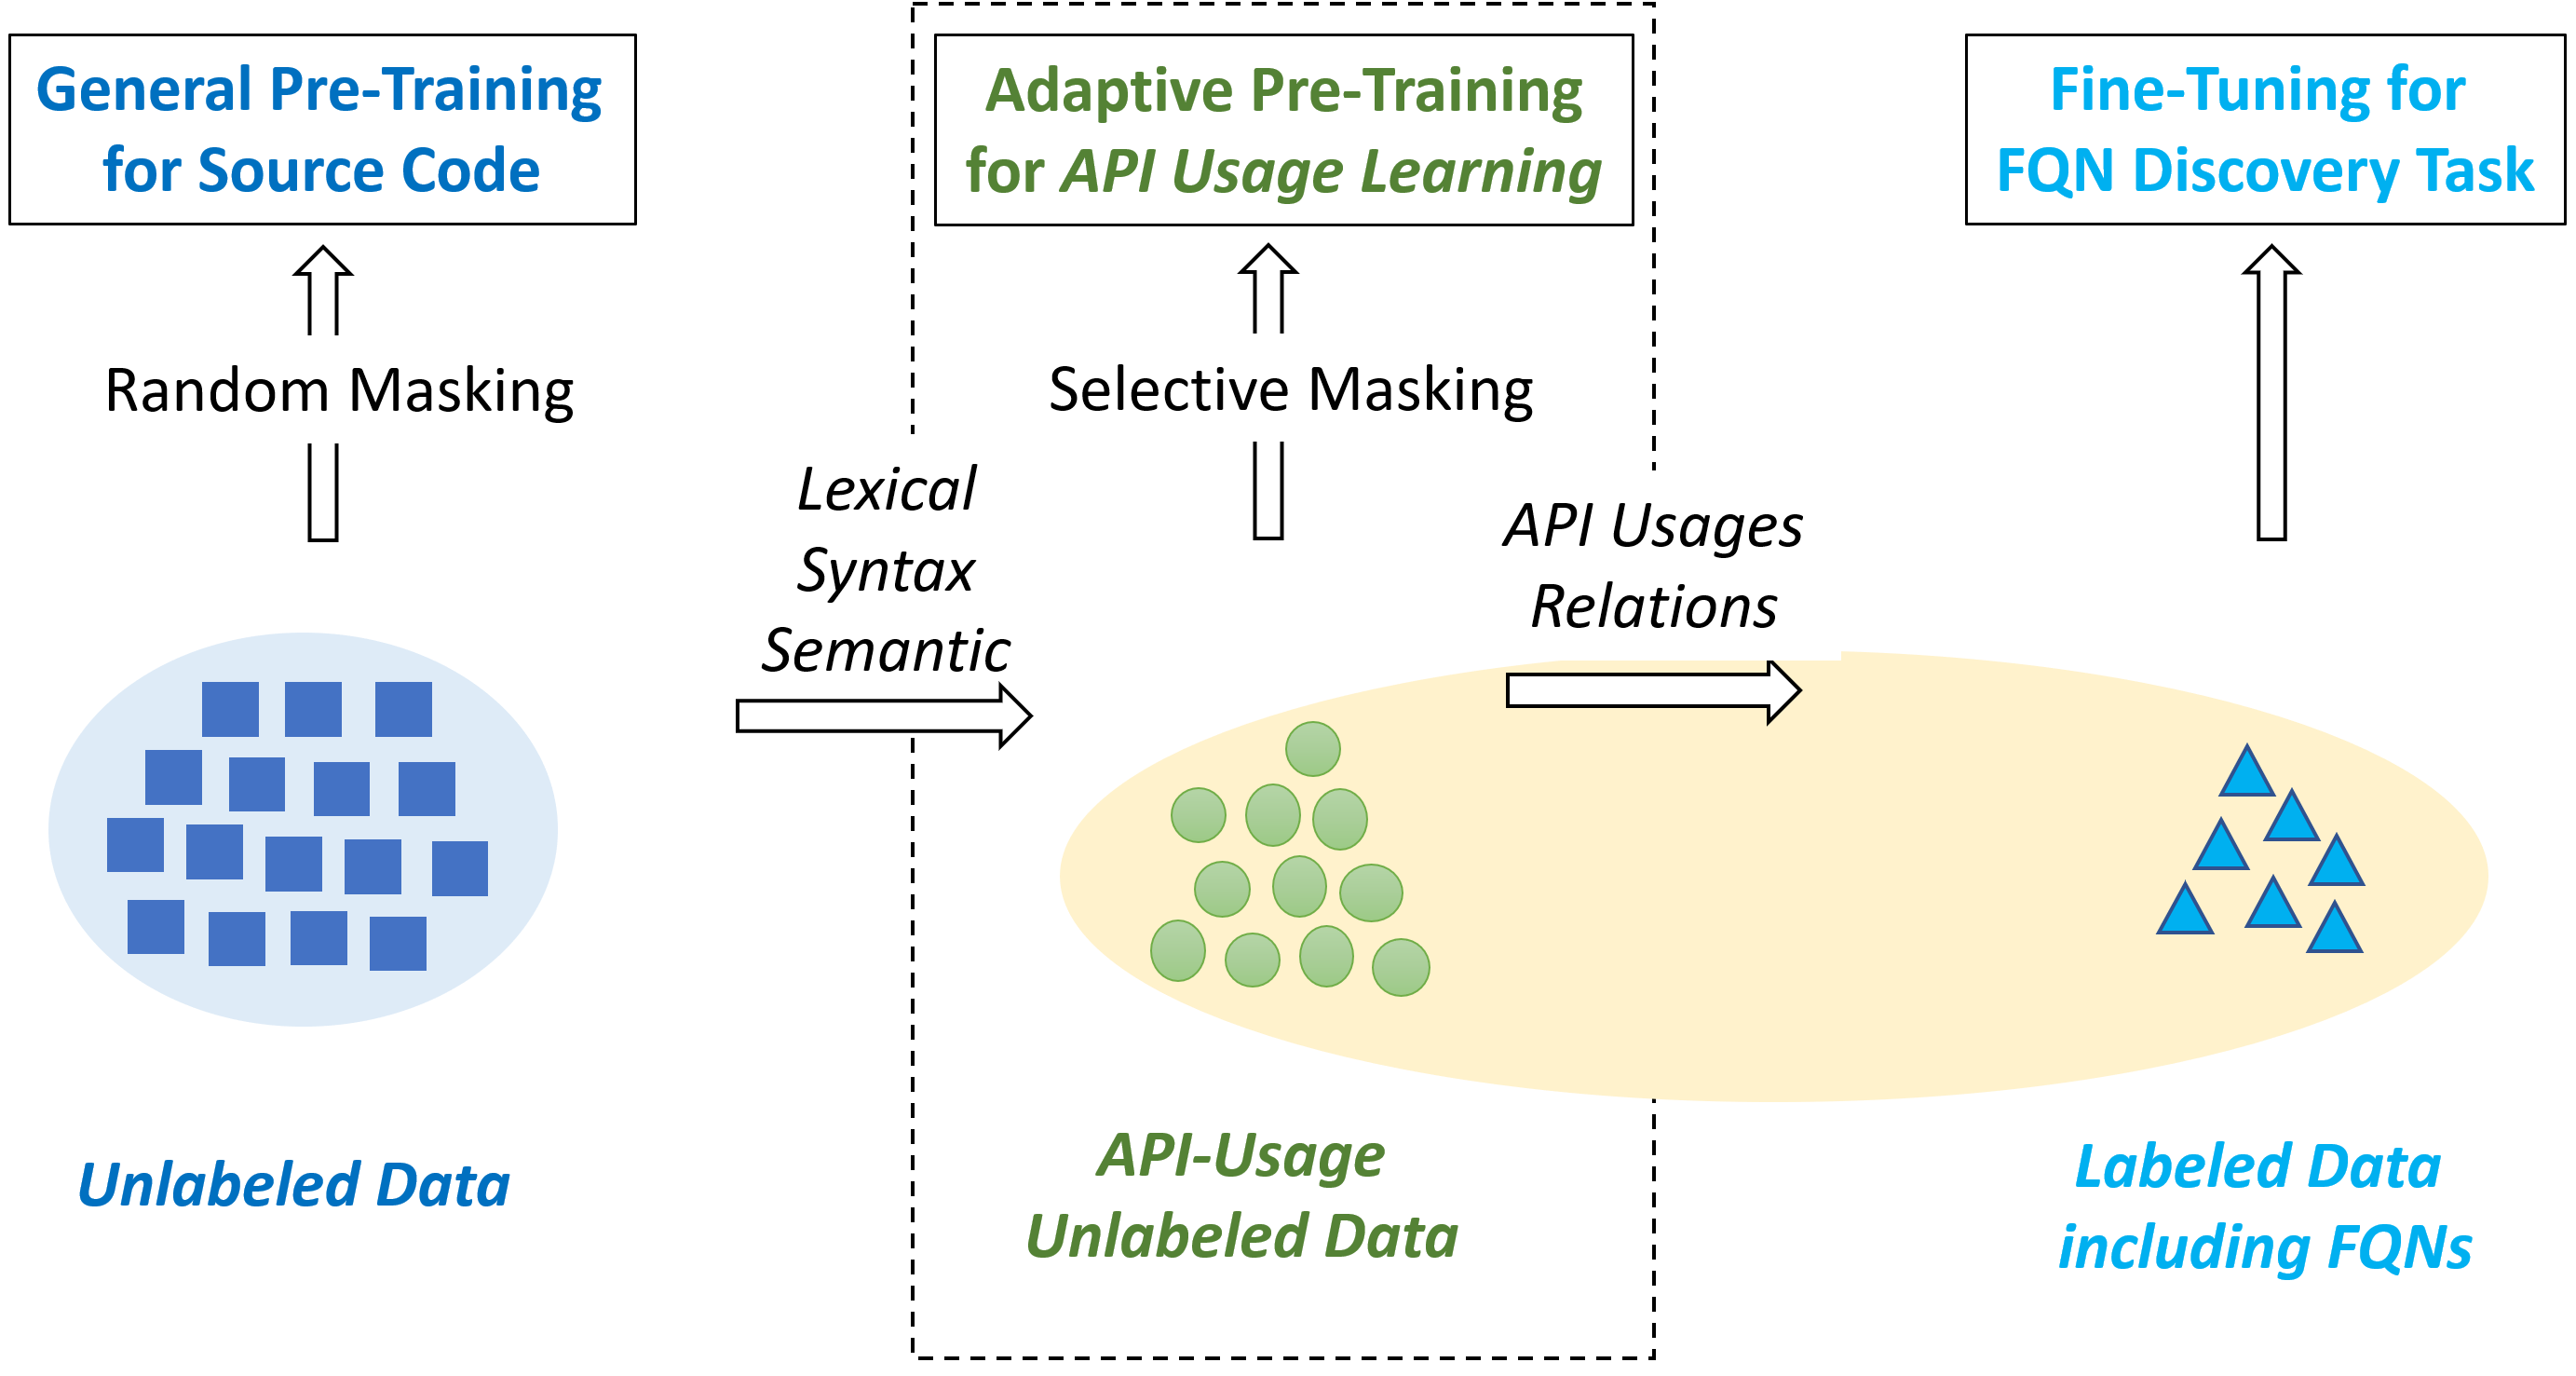
\includegraphics[width=\linewidth]{overview}
%%%        \vspace{-12pt}
%%%	\caption{{\tool} Overview with FQN-Guided Pre-Training}
%%%	\label{fig:overview}
%%%\end{figure}
%%%
%%%Figure~\ref{fig:overview} shows {\tool}'s overview. The
%%%state-of-the-art approaches in using pre-training language models
%%%often follow the pre-train-then-fine-tuning paradigm. The pre-training
%%%is task-agnostic and the fine-tuning usually suffers from the
%%%insufficient supervised training data. In {\tool}, inspiring by Gu
%%%{\em et al.}~\cite{gu-emnlp20}, we use a three-stage solution with the
%%%addition of the task-guided pre-training stage. We dedicate the
%%%task-guided pre-training stage {\em to learning API usage patterns} to
%%%help with the fully-qualified name detection task.
%%%
%%%The first stage is dedicated to the general pre-training on source
%%%code to help {\tool} learn the general lexical, syntax, and semantic
%%%characteristics of source code. For this purpose, we use
%%%CodeBERT~\cite{codebert} in which we randomly mask 15\% tokens and
%%%train the model to reconstruct the original code tokens.
%%%
%%%The second stage is aimed to effectively and efficiently learn the
%%%{\em API usage patterns} and {\em the dependencies among API elements
%%%  and the relevant program elements} in source code. From the source
%%%code without any labels (unlabeled data), we apply a selective masking
%%%strategy to focus on masking the important tokens for the FQN
%%%discovery task. From the motivation and key ideas, we identify as
%%%important the tokens corresponding to the API elements and relevant
%%%program entities via the API usage relations/dependencies. Note that
%%%the training data at this stage unlabeled as in the general
%%%pre-training stage. We expect that the model will learn the API usage
%%%patterns and relations among the code elements that complement to the
%%%general knowledge learned from the general pre-training stage. The
%%%details on our selective masking are presented later.
%%%
%%%The fine-tuning stage is dedicated to the task of recovering the FQNs
%%%in source code. It will be trained with the labeled data, i.e., with
%%%the FQNs. We can obtain such labeled data by running a program
%%%analysis tool or a compiler on a complete code.

%with the masking process that emphasizes on learning API usages and
%patterns with the unsupervised data on the dependencies/relations
%among API elements and relevant program elements.
